\section{Discrete-Time-Systems}
Ein Discrete-Time-System ist ein System, welches eine Eingangssequenz in eine Ausgangssequenz transformiert.

\subsection{Stabilität und Kausalität}
Es kann gezeigt werden, dass für ein LTI System die Impulsantwort absolut Summierbar sein muss.
\[
\sum_{n=-\infty}^{\infty}\left|h(n)\right| \lt \infty
\]

\begin{center}
	\includegraphics[width=\columnwidth]{Images/kausalität}
\end{center}



\subsection{Convolution}
\textbf{Convolution Table}\script{S126}
\begin{center}
	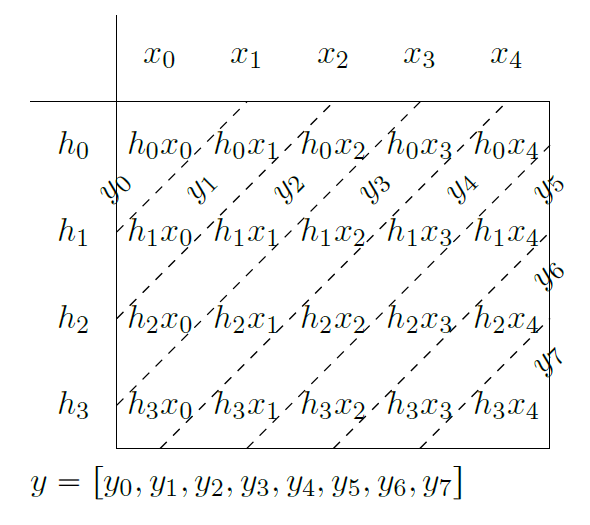
\includegraphics[width=0.7\columnwidth]{Images/convtable}
\end{center}


\textbf{LTI Form}\script{S127}
\begin{center}
	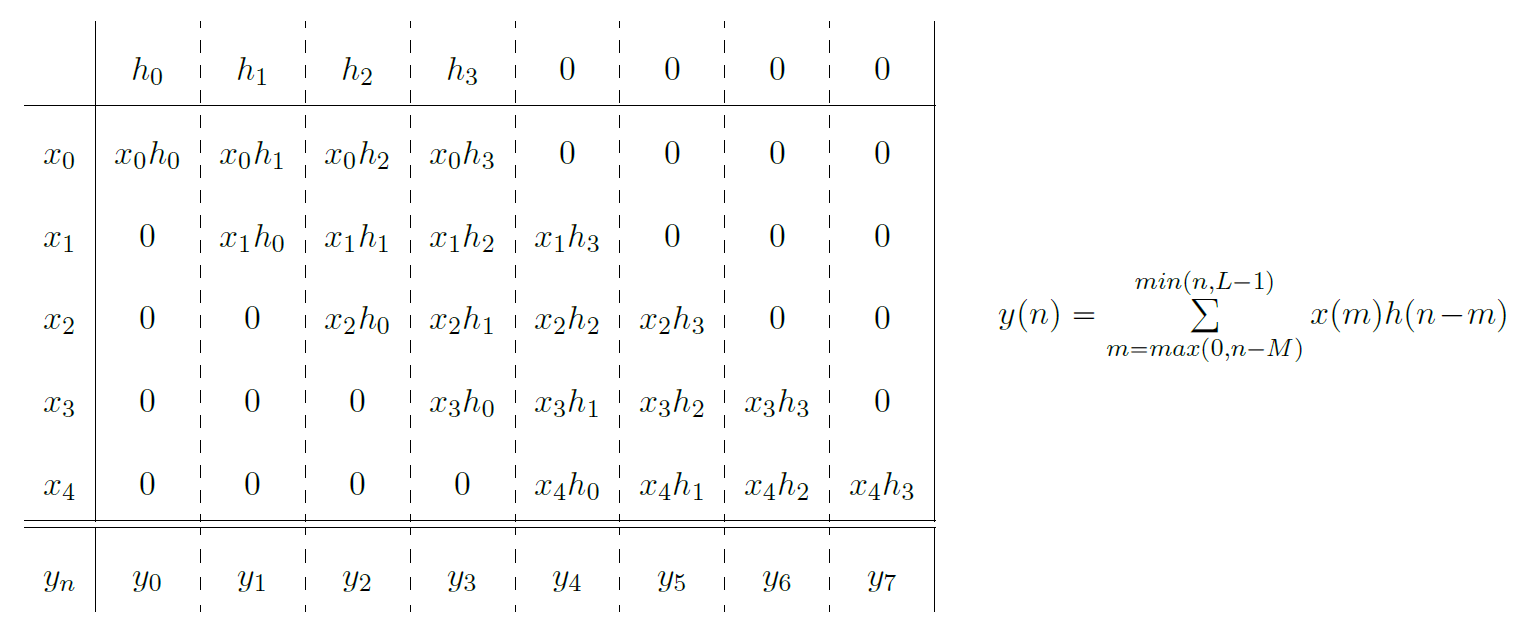
\includegraphics[width=\columnwidth]{Images/lti}
\end{center}

\textbf{Matrix Form}\script{S129}
\[
y = Hx \quad \text{oder} \quad y = Xh
\]
\begin{center}
	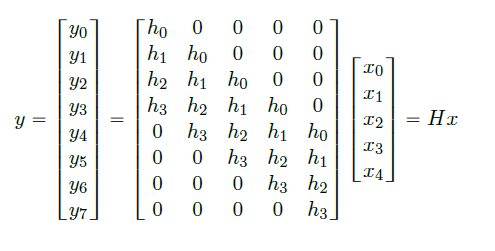
\includegraphics[width=0.7\columnwidth]{Images/matrix}
\end{center}

\textbf{Overlap Form}\script{S143}
\begin{center}
	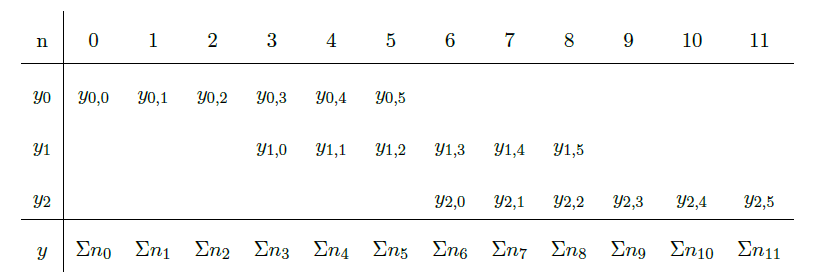
\includegraphics[width=\columnwidth]{Images/overlap}
\end{center}


\subsection{Matlab fft}
die FFT von Matlab ist eine zirkuläre Convolution implementation. Das bedeutet, dass die Transienten beim Stady-State überlagert und addiert werden müssen. Der Ausgang $y$ ist gleich lange wie der Eingang $x$!
\textbf{Beispiel}:
$x=[1, 2, 3, 4]$ und Impuls Antwort $y=[1, 0, 0, 1]$. Die ergibt sich mit der Convolution Table zu $y=[1, 2, 3, 5, 2, 3, 4]$ Dabei sind die Transienten wie folgt:
\[
y=[\underbrace{1, 2, 3}_{on}, 5, \underbrace{2, 3, 4}_{off}]
\]

Mit dem Matlab befehl $ifft(fft(x).*fft(h))$ ergibt sich
\begin{table}[H]
	\begin{tabular}{lllllllllll}
		& \multicolumn{1}{l|}{}  & \multicolumn{3}{c|}{on}                                                           & \multicolumn{1}{l|}{}     & \multicolumn{3}{c|}{off}       &   &     \\ \cline{3-9}
		& \multicolumn{1}{l|}{}  & 1                         & 2                         & 3                         & 5                         & 2 & 3 & \multicolumn{1}{l|}{4} &   &     \\
		... & \multicolumn{1}{l|}{5} & 2                         & 3                         & 4                         &                           & 1 & 2 & \multicolumn{1}{l|}{3} & 5 & ... \\ \cline{3-9}
		& \multicolumn{1}{l|}{}  & \cellcolor[HTML]{67FD9A}3 & \cellcolor[HTML]{67FD9A}5 & \cellcolor[HTML]{67FD9A}7 & \cellcolor[HTML]{67FD9A}5 & 3 & 5 & \multicolumn{1}{l|}{7} &   &     \\
		&                        &                           &                           &                           &                           &   &   &                        &   &    
	\end{tabular}
\end{table}
